% ------------------------------------------------------------------------------
% TYPO3 CMS 7.0 - What's New (German Version)
%
% @author	Patrick Lobacher <patrick@lobacher.de>
% @license	Creative Commons BY-NC-SA 3.0
% @link		http://typo3.org/download/release-notes/whats-new/
% @language	German
% ------------------------------------------------------------------------------

% change the default aspect ratio and frame size
% \documentclass[aspectratio=43]{beamer}
%
% specify vertical top alignment globally by the [t] class option:
% \documentclass[t]{beamer}
%
% for single frames, use the same option locally:
% \begin{frame}[t] ... \end{frame}

\documentclass[t]{beamer}

% suppress navigation bar
\beamertemplatenavigationsymbolsempty

\mode<presentation>
{
	\usetheme{typo3slides}
}

% global variables
\title{TYPO3 CMS 7.0 - What's New}
\subtitle{Übersicht der neuen Funktionen, Änderungen\newline und Verbesserungen}
\author{
	\centerline{Patrick Lobacher und Michael Schams}
}
\date{\today}

\begin{document}

% select TYPO3 Share font
\sharefont

% ------------------------------------------------------------------------------
% Title Page
% ------------------------------------------------------------------------------

\begingroup
	\setbeamercolor{normal text}{fg=white,bg=typo3orange}
	\setbeamercolor{title}{fg=white}
	\setbeamercolor{author}{fg=white}
	\setbeamertemplate{footline}[default]
	\begin{frame}
		\titlepage
	\end{frame}
\endgroup

% ------------------------------------------------------------------------------
% Table of Contents
% ------------------------------------------------------------------------------

\section*{TYPO3 CMS 7.0 - What's New}
\begin{frame}[fragile]
	\frametitle{Kapitelübersicht}
	\framesubtitle{Kapitelübersicht}

	\begin{multicols}{2}
		\tableofcontents
	\end{multicols}

\end{frame}

% ------------------------------------------------------------------------------
% LTXE-CHAPTER-INCLUDE:	947f71fe-f93742b1-4879d61a-4a9bbcd6
% ------------------------------------------------------------------------------

% ------------------------------------------------------------------------------
% TYPO3 CMS 8.4 - What's New - Chapter "Introduction" (Italian Version)
%
% @author	Michael Schams <schams.net>
% @license	Creative Commons BY-NC-SA 3.0
% @link		http://typo3.org/download/release-notes/whats-new/
% @language	English
% ------------------------------------------------------------------------------
% LTXE-CHAPTER-UID:		7fdf26cc-362160ab-d6c8b905-19722b20
% LTXE-CHAPTER-NAME:	Introduction
% ------------------------------------------------------------------------------

\section{Introduzione}
\begin{frame}[fragile]
	\frametitle{Introduzione}

	\begin{center}\huge{Introduzione}\end{center}
	\begin{center}\huge{\color{typo3darkgrey}\textbf{I fatti in breve}}\end{center}

\end{frame}

% ------------------------------------------------------------------------------
% LTXE-SLIDE-START
% LTXE-SLIDE-UID:		36bbd1e7-b70470c2-e4557331-e851ab9a
% LTXE-SLIDE-ORIGIN:	344cc625-72176049-0721f1aa-0580f11a English
% LTXE-SLIDE-TITLE:		TYPO3 CMS 8.4 - The Facts
% ------------------------------------------------------------------------------
\begin{frame}[fragile]
	\frametitle{Introduzione}
	\framesubtitle{TYPO3 CMS 8.4 - I fatti in breve}

	\begin{itemize}
		\item Data di rilascio: 18 Ottobre 2016
		\item Tipo di rilascio: Sprint Release
		\item Slogan: Fueling
	\end{itemize}

	\begin{figure}
		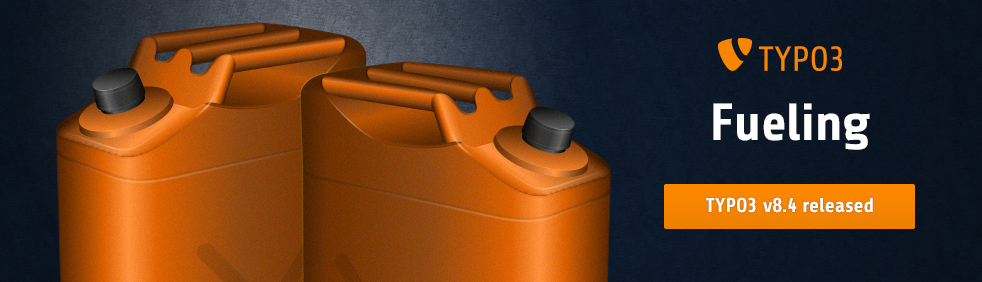
\includegraphics[width=0.95\linewidth]{Introduction/typo3cms84-banner.jpg}
	\end{figure}

\end{frame}

% ------------------------------------------------------------------------------
% LTXE-SLIDE-START
% LTXE-SLIDE-UID:		c34db54f-5ce84e64-993b5283-bd1414c5
% LTXE-SLIDE-ORIGIN:	59b04868-09a761b3-0c7ca4c3-ce6e31bb English
% LTXE-SLIDE-TITLE:		System Requirements
% ------------------------------------------------------------------------------
\begin{frame}[fragile]
	\frametitle{Introduzione}
	\framesubtitle{Requisiti di sistema}

	\begin{itemize}
		\item PHP:\tabto{2.2cm}versione 7
		\item MySQL:\tabto{2.2cm}versione da 5.5 a 5.7
		\item Spazio disco:\tabto{2.2cm}min 200 MB
		\item Impostazioni PHP:

			\begin{itemize}
				\item \texttt{memory\_limit} >= 128M
				\item \texttt{max\_execution\_time} >= 240s
				\item \texttt{max\_input\_vars} >= 1500
				\item l'opzione di compilazione \texttt{-}\texttt{-disable-ipv6} \underline{non} deve essere usata
			\end{itemize}

		\item Il Backend richiede Microsoft Internet Explorer 11 o superiore,
			Microsoft Edge, Google Chrome, Firefox, Safari o altro browser recente
			e compatibile

	\end{itemize}

\end{frame}

% ------------------------------------------------------------------------------
% LTXE-SLIDE-START
% LTXE-SLIDE-UID:		6d7a088e-555bc078-1d2027f1-5046d232
% LTXE-SLIDE-ORIGIN:	41f1b51a-6b837f9d-c4aa9584-66f8e47f English
% LTXE-SLIDE-TITLE:		Development And Release Timeline
% ------------------------------------------------------------------------------
\begin{frame}[fragile]
	\frametitle{Introduzione}
	\framesubtitle{Sviluppo e tempi di rilascio}

	\begin{figure}
		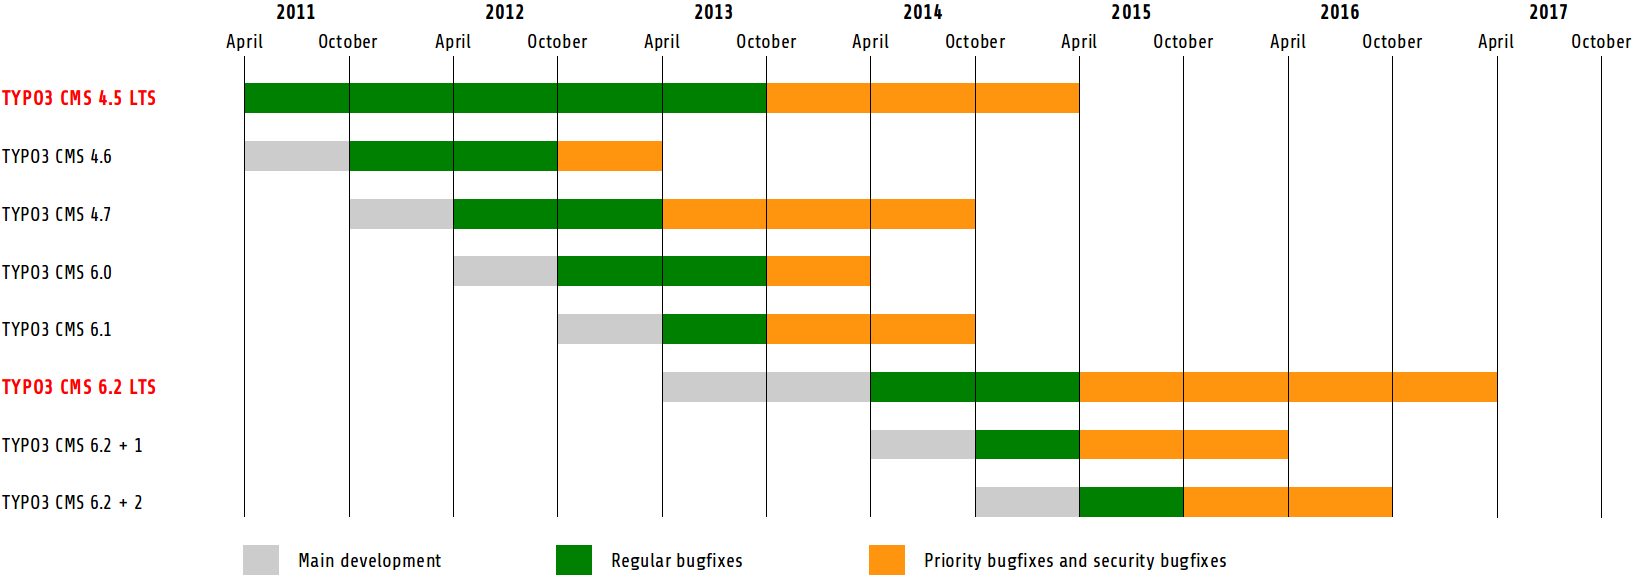
\includegraphics[width=1\linewidth]{Introduction/ReleaseAgenda.png}
	\end{figure}

\end{frame}

% ------------------------------------------------------------------------------
% LTXE-SLIDE-START
% LTXE-SLIDE-UID:		ef57635b-0d6818d0-bc469ed4-3c810ae4
% LTXE-SLIDE-ORIGIN:	f7c981ac-f359aac8-f8799a73-2adc6532 English
% LTXE-SLIDE-TITLE:		TYPO3 CMS Roadmap
% ------------------------------------------------------------------------------
\begin{frame}[fragile]
	\frametitle{Introduzione}
	\framesubtitle{TYPO3 CMS Roadmap}

	Date di rilascio stimate e loro obiettivo principale:

	\begin{itemize}

		\item v8.0 \tabto{1.1cm}22/Mar/2016\tabto{3.4cm}Aggiunta di parti dell'ultimo momento
		\item v8.1 \tabto{1.1cm}03/Mag/2016\tabto{3.4cm}Integrazione cloud
		\item v8.2 \tabto{1.1cm}05/Lug/2016\tabto{3.4cm}Prerequisiti Doctrine
		\item v8.3 \tabto{1.1cm}30/Ago/2016\tabto{3.4cm}Rich Text Editor
		\item
			\begingroup
				\color{typo3orange}
					v8.4 \tabto{1.1cm}18/Ott/2016\tabto{3.4cm}Migrazione Doctrine + Aggiornamenti
			\endgroup
		\item v8.5 \tabto{1.1cm}20/Dic/2016\tabto{3.4cm}Nuovo RTE + Supporto Integrazione
		\item v8.6 \tabto{1.1cm}14/Feb/2017\tabto{3.4cm}\textit{da determinare}
		\item v8.7 \tabto{1.1cm}04/Apr/2017\tabto{3.4cm}Preparazione LTS

	\end{itemize}

	\smaller
		\url{https://typo3.org/typo3-cms/roadmap/}\newline
		\url{https://typo3.org/news/article/kicking-off-typo3-v8-development/}
	\normalsize

\end{frame}

% ------------------------------------------------------------------------------
% LTXE-SLIDE-START
% LTXE-SLIDE-UID:		df4f964f-fa8cb997-19c5170a-4dc9c6b2
% LTXE-SLIDE-ORIGIN:	425f3f15-1178ed7e-f26438f9-a79ad9e9 English
% LTXE-SLIDE-TITLE:		Installation
% ------------------------------------------------------------------------------
\begin{frame}[fragile]
	\frametitle{Introduzione}
	\framesubtitle{Installazione}

	\begin{itemize}
		\item Procedura ufficiale di installazione su Linux/Mac OS X\newline
			(Directory Root ad esempio \texttt{/var/www/site/htdocs}):
		\begin{lstlisting}
			$ cd /var/www/site
			$ wget --content-disposition get.typo3.org/8.4
			$ tar xzf typo3_src-8.4.1.tar.gz
			$ cd htdocs
			$ ln -s ../typo3_src-8.4.1 typo3_src
			$ ln -s typo3_src/index.php
			$ ln -s typo3_src/typo3
			$ touch FIRST_INSTALL
		\end{lstlisting}

		\item Link simbolici in Microsoft Windows:

			\begin{itemize}
				\item Usa \texttt{junction} in Windows XP/2000
				\item Usa \texttt{mklink} in Windows Vista e Windows 7
			\end{itemize}

	\end{itemize}
\end{frame}

% ------------------------------------------------------------------------------
% LTXE-SLIDE-START
% LTXE-SLIDE-UID:		e38ae238-c1d61e71-6406f3e1-8f93121d
% LTXE-SLIDE-ORIGIN:	061ecffe-6aadad2d-6e64a67a-3c50a5cf English
% LTXE-SLIDE-TITLE:		Upgrade to TYPO3 CMS 7
% ------------------------------------------------------------------------------
\begin{frame}[fragile]
	\frametitle{Introduzione}
	\framesubtitle{Aggiornamento a TYPO3 CMS 8.x}

	\begin{itemize}
		\item Aggiornamenti possibili solo da TYPO3 CMS 7.6 LTS
		\item TYPO3 CMS < 7.6 LTS deve essere prima aggiornato a TYPO3 CMS 7.6 LTS
	\end{itemize}

	\begin{itemize}

		\item Istruzioni per l'aggiornamento:\newline
			\smaller\url{http://wiki.typo3.org/Upgrade#Upgrading_to_8.3}\normalsize
		\item Guida ufficiale TYPO3 "TYPO3 Installation and Upgrading":
			\smaller\url{http://docs.typo3.org/typo3cms/InstallationGuide}\normalsize
		\item Approcio generale:
			\begin{itemize}
				\item Verifica i requisiti minimi di sistema \small(PHP, MySQL, etc.)
				\item Verifica \textbf{deprecation\_*.log} nella vecchia istanza TYPO3
				\item Aggiorna tutte le estensioni all'ultima versione
				\item Imposta il nuovo sorgente ed esegui Install Tool -> Upgrade Wizard
				\item Verifica il modulo di startup per gli utenti di backend (opzionale)
			\end{itemize}
	\end{itemize}

\end{frame}

% ------------------------------------------------------------------------------

% ------------------------------------------------------------------------------
% LTXE-SLIDE-START
% LTXE-SLIDE-UID:		5449eaf9-054a9da9-8cccada5-eb6655ca
% LTXE-SLIDE-ORIGIN:	560abc87-898d82d3-b9e35f84-e348c121 English
% LTXE-SLIDE-TITLE:		PHP Version 7
% ------------------------------------------------------------------------------
\begin{frame}[fragile]
	\frametitle{Introduzione}
	\framesubtitle{PHP Version 7}

	\begin{itemize}

		\item PHP 7.0 è un requisito minimo per TYPO3 CMS 8.x
		\item TYPO3 supporterà i successivi rilasci di PHP 7 mano a mano che saranno pubblicati
		\item Questa versione fornisce un significativo incremento delle prestazioni del sistema

		\item Non solo gli editori di backend noteranno un interfaccia più veloce, ma il tempo
			di caricamento di un intera pagina di frontend in cache è inferiore a
			7 millisecondi, che è circa il 40\% più veloce paragonandolo
			allo stesso sito web con PHP versione 5.5

		\item Si sono iniziate ad utilizzare anche le nuove funzioni di questa versione di PHP,
			per esempio i generatori crittografici pseudo-casuali sono già in uso.

	\end{itemize}

\end{frame}

% ------------------------------------------------------------------------------


% ------------------------------------------------------------------------------
% LTXE-CHAPTER-INCLUDE:	e7264f0e-3f82290d-94c50cda-fb2d8e66
% ------------------------------------------------------------------------------

% ------------------------------------------------------------------------------
% TYPO3 CMS 8.1 - What's New (English Version)
%
% @author	Patrick Lobacher <patrick@lobacher.de> and Michael Schams <schams.net>
% @license	Creative Commons BY-NC-SA 3.0
% @link		http://typo3.org/download/release-notes/whats-new/
% @language	English
% ------------------------------------------------------------------------------
% LTXE-CHAPTER-UID:		dcfe6009-2200ad81-816c2edb-1f54c687
% LTXE-CHAPTER-NAME:	Backend User Interface
% ------------------------------------------------------------------------------

\section{Interfaccia utente Backend}
\begin{frame}[fragile]
	\frametitle{Interfaccia utente Backend}

	\begin{center}\huge{Capitolo 1:}\end{center}
	\begin{center}\huge{\color{typo3darkgrey}\textbf{Interfaccia utente Backend}}\end{center}

\end{frame}

% ------------------------------------------------------------------------------
% LTXE-SLIDE-START
% LTXE-SLIDE-UID:		e75a9c1e-b3d6f3ba-5c9edc92-c926d4c0
% LTXE-SLIDE-ORIGIN:	5d3d70fa-92a2935e-f1cbdc1e-285ec842 English
% LTXE-SLIDE-TITLE:		Feature: #75497 - inline backend layout wizard
% LTXE-SLIDE-REFERENCE:	!Feature-75497-InlineBackendLayoutWizard.rst
% ------------------------------------------------------------------------------
\begin{frame}[fragile]
	\frametitle{Interfaccia utente Backend}
	\framesubtitle{Wizard inline per Backend Layout}

	Un nuovo tipo di visualizzazione è stato aggiunto per il wizard del backend layout con il FormEngine in modalità inline
	(in TCA: \texttt{'renderType' => 'belayoutwizard'}).

	\begin{figure}
		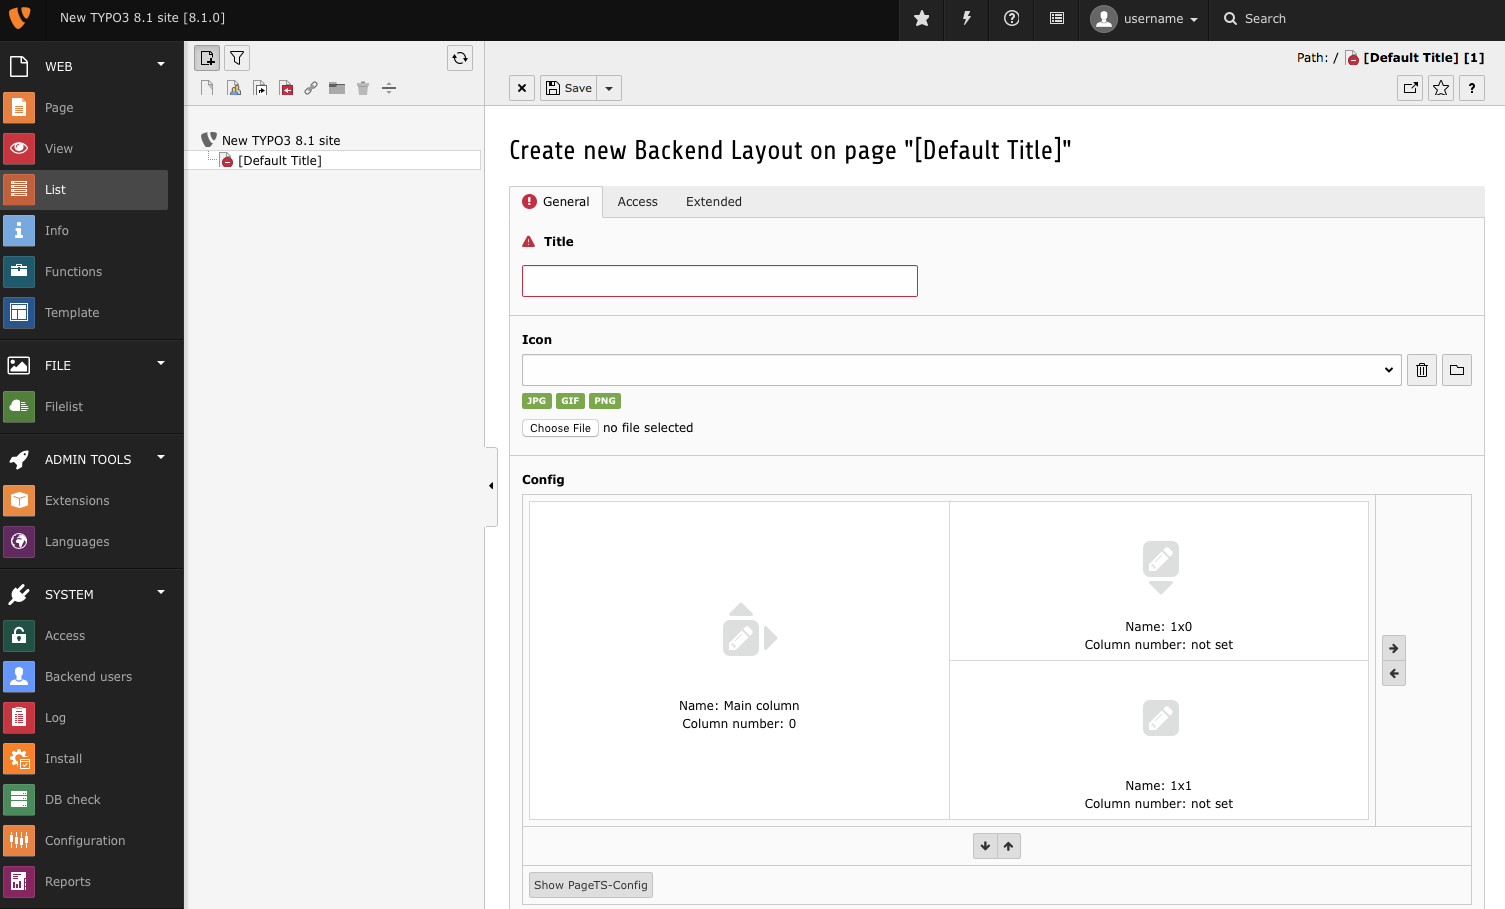
\includegraphics[width=0.70\linewidth]{BackendUserInterface/75497.png}
	\end{figure}

\end{frame}


% ------------------------------------------------------------------------------
% LTXE-SLIDE-START
% LTXE-SLIDE-UID:		7523a331-9206c084-497c0fb9-51417e20
% LTXE-SLIDE-ORIGIN:	7cab4dc0-cdfe9472-a3f0a874-dddf137d English
% LTXE-SLIDE-TITLE:		Feature: #75581 - Simplify cache clearing
% LTXE-SLIDE-REFERENCE:	!Feature-75581-SimplifyCacheClearing.rst
% ------------------------------------------------------------------------------
\begin{frame}[fragile]
	\frametitle{Interfaccia utente Backend}
	\framesubtitle{Semplificazione cancellazione Cache}

	Il sistema di cancellazione della cache è stato semplificato rimuovendo le opzioni nel menu cache clear e
	nell'Install Tool.

	\begin{itemize}

		\item \textbf{Cancellazione della cache di frontend:}\newline
			\small
				Cancellazione della cache di frontend e delle pagine relative, come prima.
			\normalsize

		\item \textbf{Cancellazione di tutte le cache:}\newline
			\small
				Cancellazione di tutte le cache di sistema, incluse le classi di caricamento, le traduzioni,
				file di configurazione delle estensioni e opcode cache. La ricostruzione di queste cache
				può impiegare un po' di tempo.
			\normalsize

	\end{itemize}

	\begin{figure}
		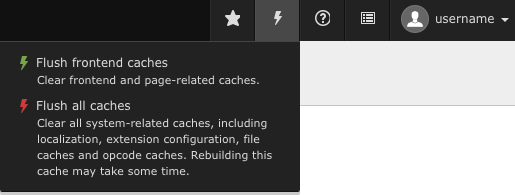
\includegraphics[width=0.45\linewidth]{BackendUserInterface/75581.png}
	\end{figure}

\end{frame}

% ------------------------------------------------------------------------------
% LTXE-SLIDE-START
% LTXE-SLIDE-UID:		e492a526-48bc139b-ef4c924c-1540678e
% LTXE-SLIDE-ORIGIN:	e24e593c-fe9bcff9-c386db3a-79491de1 English
% LTXE-SLIDE-TITLE:		Rework Workspaces (1)
% LTXE-SLIDE-REFERENCE:	Rework Workspaces
% ------------------------------------------------------------------------------
\begin{frame}[fragile]
	\frametitle{Interfaccia utente Backend}
	\framesubtitle{Rielaborazione Workspaces (1)}

	\begin{itemize}

		\item Il modulo di workspace per gestire i contenuti è stato riscritto e
			integrato molto meglio per quanto riguarda l'aspetto visivo nel backend

		\item Gli editori si renderanno conto immediatamente; esso si inserisce nel look generale
			basandosi su Twitter Bootstrap e jQuery

		\item Questo cambiamento porta anche un incremento delle prestazioni ed è un enorme passo
			avanti per un backend di TYPO3 più pulito e veloce con meno javascript.

	\end{itemize}

\end{frame}

% ------------------------------------------------------------------------------
% LTXE-SLIDE-START
% LTXE-SLIDE-UID:		b7dc1c86-39ce811a-ccd559c5-6efbf794
% LTXE-SLIDE-ORIGIN:	fe9bcff9-e24e593c-79491de1-c386db3a English
% LTXE-SLIDE-TITLE:		Rework Workspaces (2)
% LTXE-SLIDE-REFERENCE:	Rework Workspaces
% ------------------------------------------------------------------------------
\begin{frame}[fragile]
	\frametitle{Interfaccia utente Backend}
	\framesubtitle{Rielaborazione Workspaces (2)}

	Immagini del modulo di workspace:

	\begin{figure}
		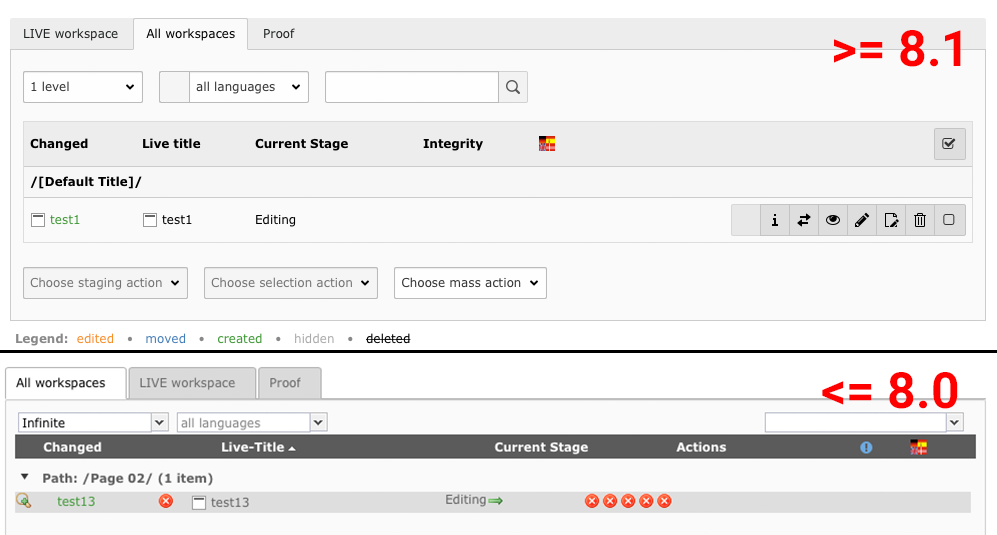
\includegraphics[width=0.85\linewidth]{BackendUserInterface/workspaces.png}
	\end{figure}

\end{frame}

% ------------------------------------------------------------------------------


% ------------------------------------------------------------------------------
% LTXE-CHAPTER-INCLUDE:	d92ab5b9-9ffa4925-30a2e34f-0d6939e5
% ------------------------------------------------------------------------------

% ------------------------------------------------------------------------------
% TYPO3 CMS 7.2 - What's New - Chapter "TypoScript" (English Version)
%
% @author	Michael Schams <schams.net>
% @license	Creative Commons BY-NC-SA 3.0
% @link		http://typo3.org/download/release-notes/whats-new/
% @language	English
% ------------------------------------------------------------------------------
% LTXE-CHAPTER-UID:		12518a77-2b90a173-4e3f8420-485e0497
% LTXE-CHAPTER-NAME:	TypoScript
% ------------------------------------------------------------------------------
% LTXE-SLIDE-START
% LTXE-SLIDE-UID:		56b025e6-cf380b11-c9d1c009-0b548d6a
% LTXE-SLIDE-TITLE:		Add flexible preview URL configuration (1)
% LTXE-SLIDE-REFERENCE:	Feature-66370-AddFlexiblePreviewUrlConfiguration.rst
% ------------------------------------------------------------------------------
\begin{frame}[fragile]
	\frametitle{TSconfig \& TypoScript}
	\framesubtitle{Flexible Preview URL Configuration (1)}

	% decrease font size for code listing
	\lstset{basicstyle=\tiny\ttfamily}

	\begin{itemize}

		\item It is now possible to configure the preview link generated for the\newline
			"save \& view" button in the backend.

		\item A common use case is to have previews for blog or news records, but you
			can also define different preview pages for normal content elements.

			\begin{lstlisting}
				TCEMAIN.preview {
				  <table name> {
				    previewPageId = 123
				    useDefaultLanguageRecord = 0
				    fieldToParameterMap {
				      uid = tx_myext_pi1[showUid]
				    }
				    additionalGetParameters {
				      tx_myext_pi1[special] = HELLO
				    }
				  }
				}
			\end{lstlisting}

	\end{itemize}

\end{frame}

% ------------------------------------------------------------------------------
% LTXE-SLIDE-START
% LTXE-SLIDE-UID:		6822c376-37649cd8-0acc836a-b856fc61
% LTXE-SLIDE-TITLE:		Add flexible preview URL configuration (2)
% LTXE-SLIDE-REFERENCE:	Feature-66370-AddFlexiblePreviewUrlConfiguration.rst
% ------------------------------------------------------------------------------
\begin{frame}[fragile]
	\frametitle{TSconfig \& TypoScript}
	\framesubtitle{Flexible Preview URL Configuration (2)}

	\begin{itemize}
		\item \texttt{previewPageId}:\newline
			\smaller
				UID of the page to use for preview\newline
				(if this setting is omitted the current page will be used)
			\normalsize
		\item \texttt{useDefaultLanguageRecord}:\newline
			\smaller
				defines if translated records will use the UID of the default record\newline
				(this is activated by default, value: 1)
			\normalsize
		\item \texttt{fieldToParameterMap}:\newline
			\smaller
				a mapping which allows to select fields of the record to be included as GET-parameters
			\normalsize
		\item \texttt{additionalGetParameters}:\newline
			\smaller
				allows to add arbitrary GET-parameters and even to override others
			\normalsize
	\end{itemize}

\end{frame}

% ------------------------------------------------------------------------------
% LTXE-SLIDE-START
% LTXE-SLIDE-UID:		c5dbf3c7-655fc6e4-227a3bf6-f5d89fb1
% LTXE-SLIDE-TITLE:
% LTXE-SLIDE-REFERENCE:	Feature-59646-AddRteConfigurationPropertyButtonsLinkTypePropertiesTargetDefault.rst
% ------------------------------------------------------------------------------
\begin{frame}[fragile]
	\frametitle{TSconfig \& TypoScript}
	\framesubtitle{RTE Configuration: Default Target}

	\begin{itemize}

		\item RTE configuration property can be used in PageTSconfig to configure a default
			target for links of a given type\newline

			\small
				\texttt{buttons.link.[}
				\textit{type}
				\texttt{].properties.target.default = ...}
			\normalsize\newline

		\item Possible link types are:\newline
			\small
				(further types may be provided by extensions)
			\normalsize

			\begin{itemize}
				\item \texttt{page}
				\item \texttt{file}
				\item \texttt{url}
				\item \texttt{mail}
				\item \texttt{spec}
			\end{itemize}
	\end{itemize}

\end{frame}

% ------------------------------------------------------------------------------
% LTXE-SLIDE-START
% LTXE-SLIDE-UID:		fd957580-301e4a0a-ad5325f5-ffa024c3
% LTXE-SLIDE-TITLE:		Strip empty HTML tags in HtmlParser
% LTXE-SLIDE-REFERENCE:	Feature-20555-StripEmptyHtmlTags.rst
% ------------------------------------------------------------------------------
\begin{frame}[fragile]
	\frametitle{TSconfig \& TypoScript}
	\framesubtitle{Strip Empty HTML Tags in HTMLparser}

	% decrease font size for code listing
	\lstset{basicstyle=\tiny\ttfamily}

	\begin{itemize}
		\item A new functionality has been implemented in the HTMLparser that allows the
			stripping of empty HTML tags

			\begin{lstlisting}
				stdWrap {
				   // this removes all empty HTML tags
				   HTMLparser.stripEmptyTags = 1
				   // this removes empty h2 and h3 tags only
				   HTMLparser.stripEmptyTags.tags = h2, h3
				}

				RTE.default.proc.entryHTMLparser_db {
				   stripEmptyTags = 1
				   stripEmptyTags.tags = p
				   stripEmptyTags.treatNonBreakingSpaceAsEmpty = 1
				}
			\end{lstlisting}

			\underline{\textbf{Note:}}
				HTMLparser strips all unknown tags by default.\newline
				Therefore it might be useful to retain these:\newline
				\texttt{HTMLparser.keepNonMatchedTags = 1}

	\end{itemize}

\end{frame}

% ------------------------------------------------------------------------------
% LTXE-SLIDE-START
% LTXE-SLIDE-UID:		62960e76-c3dca953-fe5a1070-831633fc
% LTXE-SLIDE-TITLE:		Miscellaneous
% LTXE-SLIDE-REFERENCE:	Feature-63040-AddRteConfigurationPropertyButtonsAbbreviationRemoveFieldsets.rst
% LTXE-SLIDE-REFERENCE:	commit 31c62f9311ee3d33bf792d548cc4a5fac83aa3d0
% ------------------------------------------------------------------------------
\begin{frame}[fragile]
	\frametitle{TSconfig \& TypoScript}
	\framesubtitle{Miscellaneous}

	\begin{itemize}
		\item New property \texttt{buttons.abbreviation.removeFieldsets} may be used in
			PageTSconfig to configure the abbreviation dialog

			\begin{lstlisting}
				# Possible values are:
				# acronym, definedAcronym, abbreviation, definedAbbreviation
				buttons.abbreviation.removeFieldsets = acronym,definedAcronym
			\end{lstlisting}

		\item Property \texttt{inlineLanguageLabel} of object \texttt{PAGE} can handle\newline
			\texttt{LLL:} references now

	\end{itemize}

\end{frame}

% ------------------------------------------------------------------------------


% ------------------------------------------------------------------------------
% LTXE-CHAPTER-INCLUDE:	7cb2d402-105890ae-a1632623-719adbb6
% ------------------------------------------------------------------------------

% ------------------------------------------------------------------------------
% TYPO3 CMS 7.6 - What's New - Chapter "In-Depth Changes" (Greek Version)
%
% @author	Angeliki Plati <ag.plati@gmail.com>
% @license	Creative Commons BY-NC-SA 3.0
% @link		http://typo3.org/download/release-notes/whats-new/
% @language	Greek
% ------------------------------------------------------------------------------
% LTXE-CHAPTER-UID:		7229f1b9-b481e9bc-09c46183-a86b6a7e
% LTXE-CHAPTER-NAME:	In-Depth Changes
% ------------------------------------------------------------------------------

\section{\greektext ������� �������}
\begin{frame}[fragile]
	\frametitle{\greektext ������� �������}

	\begin{center}\huge{\greektext �������� 3:}\end{center}
	\begin{center}\huge{\color{typo3darkgrey}\textbf{\greektext ������� �������}}\end{center}

\end{frame}

% ------------------------------------------------------------------------------
% LTXE-SLIDE-START
% LTXE-SLIDE-UID:		fb7f39e9-a9c3b856-0f20d933-42501d14
% LTXE-SLIDE-ORIGIN:	159a2d7f-b679989c-30cf1736-6693f827 English
% LTXE-SLIDE-TITLE:		Bootstrap for Install Tool (1)
% ------------------------------------------------------------------------------

\begin{frame}[fragile]
	\frametitle{\greektext ������� �������}
	\framesubtitle{\latintext Bootstrap \greektext ��� �� \latintext Install Tool (1)}

	\begin{itemize}

		\item \greektext �� \latintext Install Tool \greektext ��������� ���� ��� \latintext Bootstrap - \greektext
		��� �� ������� ��� ������������:

			\latintext\begin{figure}
				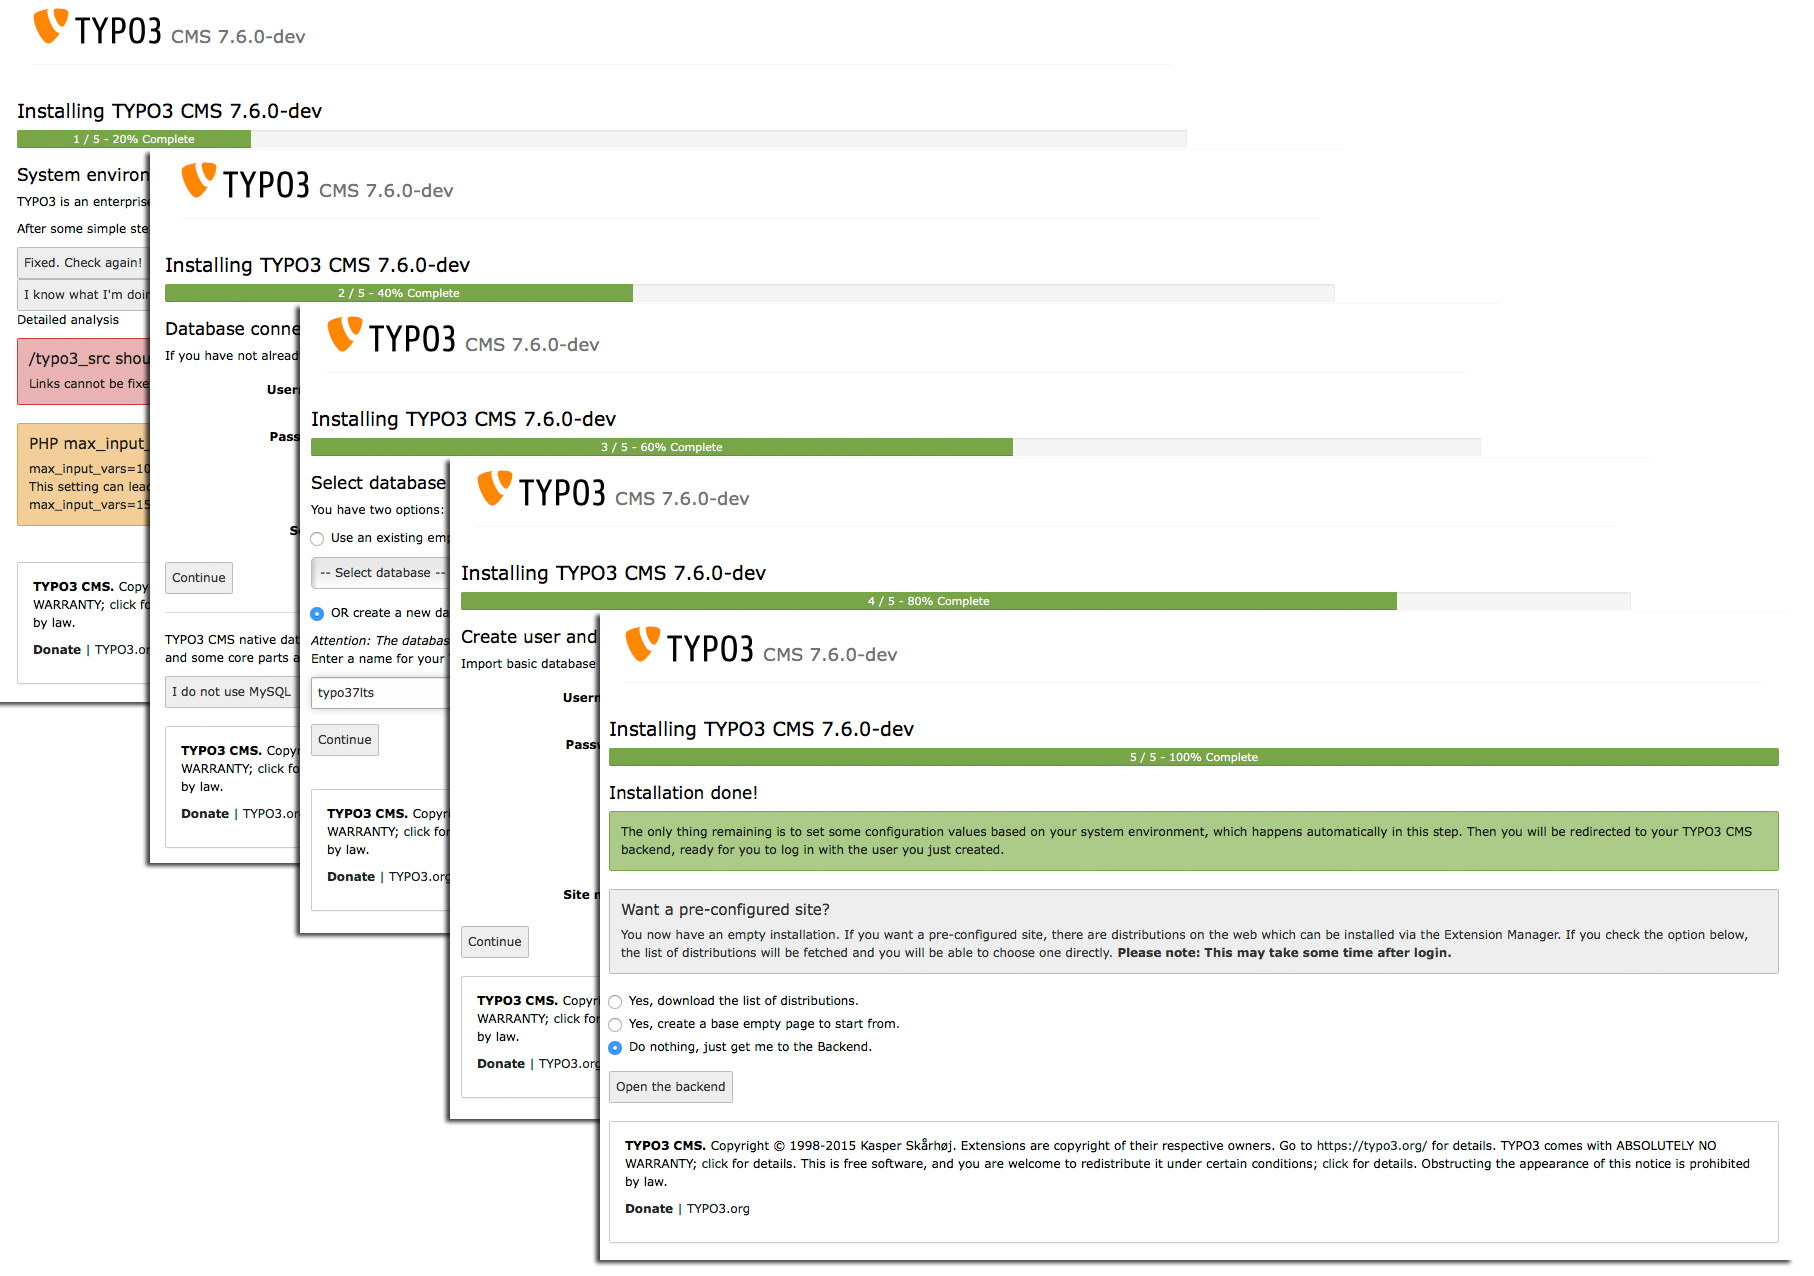
\includegraphics[width=0.7\linewidth]{InDepthChanges/InstallToolBootstrap01.jpg}
			\end{figure}

	\end{itemize}

\end{frame}

% ------------------------------------------------------------------------------
% LTXE-SLIDE-START
% LTXE-SLIDE-UID:		57b94677-df4363dd-e5477dbf-04d344c7
% LTXE-SLIDE-ORIGIN:	66a71f73-91b6c90e-e548a037-e2d47f94 English
% LTXE-SLIDE-TITLE:		Bootstrap for Install Tool (2)
% ------------------------------------------------------------------------------

\begin{frame}[fragile]
	\frametitle{\greektext ������� �������}
	\framesubtitle{\latintext Bootstrap \greektext ��� �� \latintext Install Tool (2)}

	\begin{itemize}

		\item \greektext �� \latintext Install Tool \greektext ��������� ���� ��� \latintext Bootstrap - \greektext ��� ���
		 ���������� \latintext(configuration):

			\latintext\latintext\begin{figure}
				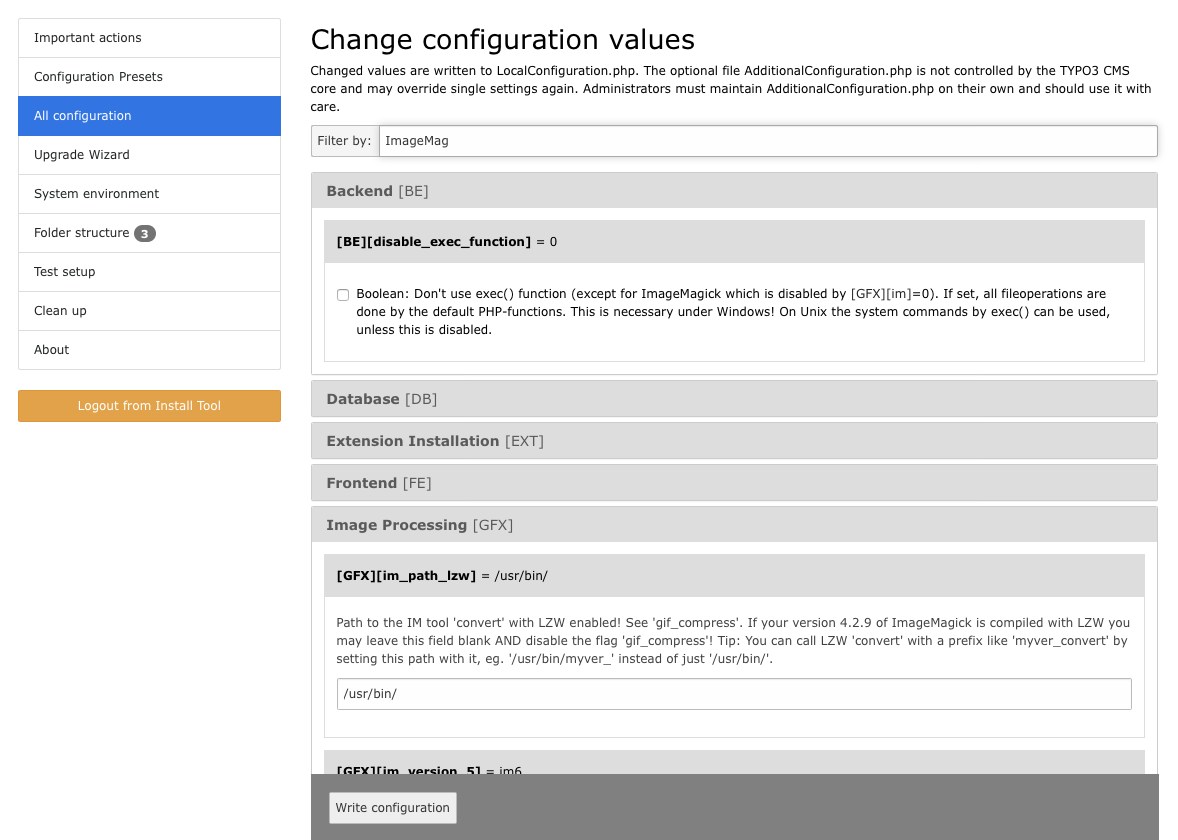
\includegraphics[width=0.7\linewidth]{InDepthChanges/InstallToolBootstrap02.png}
			\end{figure}

	\end{itemize}

\end{frame}

% ------------------------------------------------------------------------------
% LTXE-SLIDE-START
% LTXE-SLIDE-UID:		5c40f730-3d75f880-2c050954-902634a3
% LTXE-SLIDE-ORIGIN:	f901074a-4080140f-dd93e505-1e8c2178 English
% LTXE-SLIDE-ORIGIN:	d5acb2d2-159a2d7f-6693f827-30cf1736 German
% LTXE-SLIDE-TITLE:		Form protection API for frontend usage
% LTXE-SLIDE-REFERENCE:	Feature-56633-FormProtectionAPIForFrontEndUsage.rst
% ------------------------------------------------------------------------------

\begin{frame}[fragile]
	\frametitle{\greektext ������� �������}
	\framesubtitle{\greektext ��������� \latintext CSRF \greektext ��� �� \latintext Frontend Plugins}

	% decrease font size for code listing
	\lstset{basicstyle=\tiny\ttfamily}

	\begin{itemize}

		\item \greektext ��� ����� ��������� �� ����� ��� \latintext FormProtection API \greektext ��� \latintext frontend

		\item \greektext ���� �������� ��� ��������� \latintext CSRF (Cross-Site Request Forgery)

			\latintext\begin{lstlisting}
				$formToken = \TYPO3\CMS\Core\FormProtection\FormProtectionFactory::get()->getFormProtection()->generateToken('news', 'edit', $uid);
				if (
				  $dataHasBeenSubmitted
				  && \TYPO3\CMS\Core\FormProtection\FormProtectionFactory::get()->validateToken(
				    \TYPO3\CMS\Core\Utility\GeneralUtility::_POST('formToken'), 'User setup', 'edit')) {
				  // processes the data
				}
				else {
				  // invalid token!
				}
			\end{lstlisting}

	\end{itemize}

\end{frame}

% ------------------------------------------------------------------------------
% LTXE-SLIDE-START
% LTXE-SLIDE-UID:		a5c1d7d5-a793018d-2463f644-1502b46d
% LTXE-SLIDE-ORIGIN:	0198b067-68da7843-6a6d3f6d-94cee9b7 English
% LTXE-SLIDE-ORIGIN:	388c7243-b679989c-e2b30dbb-78f1aea4 German
% LTXE-SLIDE-TITLE:		Added LinkBrowser APIs (1)
% LTXE-SLIDE-REFERENCE:	Feature-66369-AddedLinkBrowserAPIs.rst
% ------------------------------------------------------------------------------

\begin{frame}[fragile]
	\frametitle{\greektext ������� �������}
	\framesubtitle{\latintext Tabs \greektext ��� ��� \latintext LinkBrowser (1)}

	% decrease font size for code listing
	\lstset{basicstyle=\tiny\ttfamily}

	\begin{itemize}

		\item \greektext ���� �� ��� ������������� ��������� ��� �������� ���
		\latintext LinkBrowser \greektext �� ��� \latintext tabs

		\item \greektext K��� \latintext tab \greektext ����� ��� �� ���������� ���� \latintext "LinkHandler", \greektext
		� ������ ������ �� �������� ��� �������� ������� \latintext (Interface):\newline
			\latintext\small
				\texttt{\textbackslash TYPO3\textbackslash CMS\textbackslash Recordlist\textbackslash LinkHandler\textbackslash LinkHandlerInterface}
			\normalsize

		\item \greektext �� \latintext LinkHandlers \greektext ����� ������������� ��� \latintext PageTSconfig \greektext �� ����:

			\latintext\begin{lstlisting}
				file {
				  handler = TYPO3\\CMS\\Recordlist\\LinkHandler\\FileLinkHandler
				  label = LLL:EXT:lang/locallang_browse_links.xlf:file
				  displayAfter = page
				  scanAfter = page
				  configuration {
				    customConfig = passed to the handler
				  }
				}
			\end{lstlisting}

	\end{itemize}

\end{frame}

% ------------------------------------------------------------------------------
% LTXE-SLIDE-START
% LTXE-SLIDE-UID:		e30adb51-b7f5a42f-e8d02ad3-b31f0cce
% LTXE-SLIDE-ORIGIN:	7ff322bc-2ace574c-34ddebb5-559fd90c English
% LTXE-SLIDE-ORIGIN:	dfd89b4b-7b4b816c-e5904ba8-2527339b German
% LTXE-SLIDE-TITLE:		Added LinkBrowser APIs (2)
% LTXE-SLIDE-REFERENCE:	Feature-66369-AddedLinkBrowserAPIs.rst
% ------------------------------------------------------------------------------

\begin{frame}[fragile]
	\frametitle{\greektext ������� �������}
	\framesubtitle{\latintext Tabs \greektext ��� ��� \latintext (2)}

	% decrease font size for code listing
	\lstset{basicstyle=\tiny\ttfamily}

	\begin{itemize}

		\item \greektext �� �������� \latintext \texttt{displayBefore} \greektext ��� \latintext \texttt{displayAfter}
		\greektext ���������� ��� ������ ��� \latintext tabs

		\item \greektext �� �������� \latintext \texttt{scanBefore} \greektext ��� \latintext \texttt{scanAfter} \greektext
		���������� �� ����� �� ��� ����� �� \latintext handlers \greektext ����������� ���� ���������� ���������� ���������

			\latintext\begin{lstlisting}
				$GLOBALS['TYPO3_CONF_VARS']['SC_OPTIONS']['LinkBrowser']['hooks'][1444048118] = [
				  'handler' => \Vendor\Ext\MyClass::class,
				  'before' => [], // optional
				  'after' => [] // optional
				];
			\end{lstlisting}

	\end{itemize}

\end{frame}

% ------------------------------------------------------------------------------
% LTXE-SLIDE-START
% LTXE-SLIDE-UID:		146ef043-c98a5f26-dcc6c06d-42bf0733
% LTXE-SLIDE-ORIGIN:	1ef90646-4f4342dd-3bf0112b-95acba1b English
% LTXE-SLIDE-ORIGIN:	687f24a3-032124a3-7ac41f15-26329962 German
% LTXE-SLIDE-TITLE:		Module Template API (1)
% LTXE-SLIDE-REFERENCE:	Feature-69814-ModuleTemplateAPI.rst
% ------------------------------------------------------------------------------

\begin{frame}[fragile]
	\frametitle{\greektext ������� �������}
	\framesubtitle{Module Template API (1)}

	% decrease font size for code listing
	\lstset{basicstyle=\tiny\ttfamily}

	\begin{itemize}

		\item \greektext ��� ��� \latintext Module Template API \greektext ���� �� ����� ��� �������������� ��� ����������
		��� \latintext DocHeaders

		\item \greektext ���������� 1: �������� ���� ��������

			\latintext\begin{lstlisting}
				$openInNewWindowButton = $this->moduleTemplate->getDocHeaderComponent()->getButtonBar()
				  ->makeLinkButton()
				  ->setHref('#')
				  ->setTitle($this->getLanguageService()->sL(
				    'LLL:EXT:lang/locallang_core.xlf:labels.openInNewWindow', TRUE
				    ))
				  ->setIcon($this->iconFactory->getIcon('actions-window-open', Icon::SIZE_SMALL))
				  ->setOnClick($aOnClick);

				$this->moduleTemplate->getDocHeaderComponent()->getButtonBar()
				  ->addButton($openInNewWindowButton, ButtonBar::BUTTON_POSITION_RIGHT);
			\end{lstlisting}
	\end{itemize}

\end{frame}

% ------------------------------------------------------------------------------
% LTXE-SLIDE-START
% LTXE-SLIDE-UID:		61fbcc28-5b90c26b-1613c13c-60a90ea0
% LTXE-SLIDE-ORIGIN:	44c8e88e-5668ccb6-3cf424ea-c6a40ecf English
% LTXE-SLIDE-ORIGIN:	1570c8c9-2dfa48e9-058d2d04-bff5465d German
% LTXE-SLIDE-TITLE:		Module Template API (2)
% LTXE-SLIDE-REFERENCE:	Feature-69814-ModuleTemplateAPI.rst
% ------------------------------------------------------------------------------

\begin{frame}[fragile]
	\frametitle{\greektext ������� �������}
	\framesubtitle{Module Template API (2)}

	% decrease font size for code listing
	\lstset{basicstyle=\tiny\ttfamily}

	\begin{itemize}
		\item \greektext ���������� 2: �������� ���� ����� �� �������� �����

			\latintext\begin{lstlisting}
				$languageMenu = $this->moduleTemplate->getDocHeaderComponent()
				  ->getModuleMenuRegistry()->makeMenu()
				  ->setIdentifier('_langSelector')
				  ->setLabel($this->getLanguageService()->sL(
				    'LLL:EXT:lang/locallang_general.xlf:LGL.language', TRUE
				  ));

				$menuItem = $languageMenu->makeMenuItem()
				  ->setTitle($lang['title'] . $newTranslation)
				  ->setHref($href);

				if((int)$lang['uid'] === $currentLanguage) {
				  $menuItem->setActive(TRUE);
				}

				$languageMenu->addMenuItem($menuItem);
				$this->moduleTemplate->getDocHeaderComponent()->getModuleMenuRegistry()->addMenu($languageMenu);
			\end{lstlisting}
	\end{itemize}

\end{frame}


% ------------------------------------------------------------------------------
% LTXE-SLIDE-START
% LTXE-SLIDE-UID:		168df078-18d15bd7-9a74f411-a271e50a
% LTXE-SLIDE-ORIGIN:	2ffbc623-117a44dc-923610ec-78a3afc2 English
% LTXE-SLIDE-ORIGIN:	df3ea848-d5406e98-edbd6684-485ff477 German
% LTXE-SLIDE-TITLE:		PSR-7-based Routing for Backend AJAX Requests
% LTXE-SLIDE-REFERENCE:	Feature-69916-PSR-7-basedRoutingForBackendAJAXRequests.rst
% ------------------------------------------------------------------------------

\begin{frame}[fragile]
	\frametitle{\greektext ������� �������}
	\framesubtitle{\greektext ����������� \latintext PSR-7 \greektext ��� \latintext Backend AJAX Requests}

	% decrease font size for code listing
	\lstset{basicstyle=\tiny\ttfamily}

	\begin{itemize}

		\item \greektext ��� ��� �������� ���� ��������� ��� ��� \latintext AJAX request, \greektext �� ������
			\latintext\texttt{Configuration/Backend/AjaxRoutes.php}\newline
			\greektext ������ �� ������������ �� �� �������� �����������:

			\latintext\begin{lstlisting}
				return [
				  // do something
				  'unique_route_name' => [
				    'path' => '/toolcollection/some-action',
				    'target' => \Vendor\Controller\SomeController::class . '::myAction',
				  ]
				];
			\end{lstlisting}

	\end{itemize}

\end{frame}

% ------------------------------------------------------------------------------
% LTXE-SLIDE-START
% LTXE-SLIDE-UID:		67138f5a-0623c3ab-1acbe95a-f121e37c
% LTXE-SLIDE-ORIGIN:	b68a9d26-30e6d4a0-7bccecf2-ad1f93c6 English
% LTXE-SLIDE-ORIGIN:	cb01cca6-58e91977-d18fa0b3-cba021ab German
% LTXE-SLIDE-TITLE:		Introduced two new Hooks for OpenID (getUserRecord)
% LTXE-SLIDE-REFERENCE:	Feature-44127-HooksForOpenIdToAutomaticallyCreateUserAccounts.rst
% ------------------------------------------------------------------------------
\begin{frame}[fragile]
	\frametitle{\greektext ������� �������}
	\framesubtitle{\latintext OpenID \greektext �������� \latintext (Hook) \texttt{getUserRecord}}

	% decrease font size for code listing
	\lstset{basicstyle=\tiny\ttfamily}

	\greektext ��� �������� ����� ��������� ��� \latintext OpenID service (1/2)

		\begin{itemize}

			\item \greektext �������� 1:\newline
				\smaller\smaller
					\latintext\texttt{\$GLOBALS['TYPO3\_CONF\_VARS']['SC\_OPTIONS']['openid']['getUserRecord']}
				\normalsize

				\begin{itemize}
					\item \greektext ���������� ��� ������� ������ ���� ���� ������������, �:
					\item \greektext ���������� ��� ��� ������� �� �� ������� �����
					\item \greektext �� ���������� \latintext\texttt{record}, \texttt{response} \greektext ��� \latintext \texttt{authInfo} \greektext
					������������ ��� ��������
				\end{itemize}

		\end{itemize}

\end{frame}

% ------------------------------------------------------------------------------
% LTXE-SLIDE-START
% LTXE-SLIDE-UID:		7854fdf6-584fdd28-988ab41d-9283e206
% LTXE-SLIDE-ORIGIN:	b9b259e4-9d35ace7-edff1014-7390d1d1 English
% LTXE-SLIDE-ORIGIN:	ea0bfed8-831666d7-1ba40bb9-7a95723a German
% LTXE-SLIDE-TITLE:		Introduced two new Hooks for OpenID (authRequest)
% LTXE-SLIDE-REFERENCE:	Feature-44127-HooksForOpenIdToAutomaticallyCreateUserAccounts.rst
% ------------------------------------------------------------------------------
\begin{frame}[fragile]
	\frametitle{\greektext ������� �������}
	\framesubtitle{\greektext �������� \latintext (Hook) \texttt{authRequest}}

	% decrease font size for code listing
	\lstset{basicstyle=\tiny\ttfamily}

	\greektext ��� �������� ����� ��������� ��� \latintext OpenID service (2/2)

		\begin{itemize}

			\item \greektext �������� 2:\newline
				\latintext\smaller\smaller
					\texttt{\$GLOBALS['TYPO3\_CONF\_VARS']['SC\_OPTIONS']['openid']['authRequest']}
				\normalsize

				\begin{itemize}
					\item \greektext ���������� �� \latintext Authentication Request, \greektext ���� ���� ������
					\item \greektext ������ �� �������������� ��� �� \latintext request \greektext ������������ ���������
					���� ��� \latintext nickname \greektext ��� ��� \latintext OpenID Server \greektext ��� ����������
					\item \greektext �� ���������� \latintext \texttt{authRequest} \greektext ��� \latintext \texttt{authInfo}
					\greektext ������������ ��� ��������
				\end{itemize}

		\end{itemize}

\end{frame}

% ------------------------------------------------------------------------------
% LTXE-SLIDE-START
% LTXE-SLIDE-UID:		d6cd9df0-bd81dbae-51c9a744-7f157bb5
% LTXE-SLIDE-ORIGIN:	1626edc6-8d93ff84-f64178bf-8e7650df English
% LTXE-SLIDE-ORIGIN:	115a4459-3653bb99-1680d6ab-d8c3c69b German
% LTXE-SLIDE-TITLE:		Hook in BackendUserAuthentication::getDefaultUploadFolder (1)
% LTXE-SLIDE-REFERENCE:	Feature-68895-IntroducedHookInBackendUserAuthenticationgetDefaultUploadFolder.rst
% ------------------------------------------------------------------------------
\begin{frame}[fragile]
	\frametitle{\greektext ������� �������}
	\framesubtitle{\greektext �������� ��� ������ (1)}

	% decrease font size for code listing
	\lstset{basicstyle=\tiny\ttfamily}

	\begin{itemize}

		\item \greektext ����� ���� ������ �� ������� ������ ��� ������ \latintext upload \greektext
		 ��� ������������ ��� ��� \latintext
			\texttt{BackendUserAuthentication::getDefaultUploadFolder()}

		\item \greektext � ������� ��� ��������� ��� ������ \latintext \texttt{ext\_localconf.php} \greektext ������� �� ����:

			\latintext\begin{lstlisting}
				$GLOBALS['TYPO3_CONF_VARS']['SC_OPTIONS']['t3lib/class.t3lib_userauthgroup.php']
				  ['getDefaultUploadFolder'][] =
				  \Vendor\MyExtension\Hooks\DefaultUploadFolder::class . '->getDefaultUploadFolder';
			\end{lstlisting}

	\end{itemize}

\end{frame}

% ------------------------------------------------------------------------------
% LTXE-SLIDE-START
% LTXE-SLIDE-UID:		e3b6ef85-9b24f220-ee6cb871-28d33337
% LTXE-SLIDE-ORIGIN:	9c150d50-ee3ba19b-120ef653-e714135c English
% LTXE-SLIDE-ORIGIN:	d1041967-32814ee3-2172e570-4a6d21bd German
% LTXE-SLIDE-TITLE:		Hook in BackendUserAuthentication::getDefaultUploadFolder (2)
% LTXE-SLIDE-REFERENCE:	Feature-68895-IntroducedHookInBackendUserAuthenticationgetDefaultUploadFolder.rst
% ------------------------------------------------------------------------------
\begin{frame}[fragile]
	\frametitle{\greektext ������� �������}
	\framesubtitle{\greektext �������� ��� ������ (2)}

	% decrease font size for code listing
	\lstset{basicstyle=\tiny\ttfamily}

	\small \greektext ����������:\normalsize

		\latintext\begin{lstlisting}
			<?php
			namespace Vendor\MyExtension\Hooks;
			use TYPO3\CMS\Core\Authentication\BackendUserAuthentication;
			use TYPO3\CMS\Core\Resource\Folder;

			/**
			 * Class DefaultUploadFolder
			 */
			class DefaultUploadFolder {

			  /**
			   * Get default upload folder
			   * If there is a folder present with the same name as the last part of the table name use that folder.
			   * @param array $params
			   * @param BackendUserAuthentication $backendUserAuthentication
			   * @return Folder
			   */
			   public function getDefaultUploadFolder($params, BackendUserAuthentication $backendUserAuthentication) {
			    [...]
		\end{lstlisting}

\end{frame}

% ------------------------------------------------------------------------------
% LTXE-SLIDE-START
% LTXE-SLIDE-UID:		3403e92e-1bb3a37a-b53a812c-c1b7bbdb
% LTXE-SLIDE-ORIGIN:	a4d7bec0-6c19d8b2-6a6be951-5d5aa0c0 English
% LTXE-SLIDE-ORIGIN:	2f855107-2262065c-c865f953-91b4f0ea German
% LTXE-SLIDE-TITLE:		Hook in BackendUserAuthentication::getDefaultUploadFolder (3)
% LTXE-SLIDE-REFERENCE:	Feature-68895-IntroducedHookInBackendUserAuthenticationgetDefaultUploadFolder.rst
% ------------------------------------------------------------------------------
\begin{frame}[fragile]
	\frametitle{\greektext ������� �������}
	\framesubtitle{\greektext �������� ��� ������ (3)}

	% decrease font size for code listing
	\lstset{basicstyle=\tiny\ttfamily}

	\small \greektext ���������� (��������):\normalsize

		\latintext\begin{lstlisting}
			    [...]

			    /** @var Folder $uploadFolder */
			    $uploadFolder = $params['uploadFolder'];
			    $pid = $params['pid'];
			    $table = $params['table'];
			    $field = $params['field'];

			    $matches = [];
			    if (!empty($uploadFolder) && preg_match('/_([a-z]+)$/', $table, $matches)) {
			      $folderName = $matches[1];
			      if ($uploadFolder->hasFolder($folderName)) {
			        $uploadFolder = $uploadFolder->getSubfolder($folderName);
			      }
			    }
			    return $uploadFolder;
			  }
			}
		\end{lstlisting}

\end{frame}

% ------------------------------------------------------------------------------
% LTXE-SLIDE-START
% LTXE-SLIDE-UID:		498d8f09-18df23db-2a659e1c-cf467bca
% LTXE-SLIDE-ORIGIN:	2c656d9e-38b9be7a-d590cb6e-21eccd4d English
% LTXE-SLIDE-ORIGIN:	cd6ba83d-9f068dee-b8887ffa-4a2eff29 German
% LTXE-SLIDE-TITLE:		Diverse ?nderungen
% LTXE-SLIDE-REFERENCE:	Deprecation-69822-DeprecateSelectFieldTca.rst
% ------------------------------------------------------------------------------
\begin{frame}[fragile]
	\frametitle{\greektext ������� �������}
	\framesubtitle{\greektext �������}

	\begin{itemize}

		\item \greektext � ����� ��� ����� ������ \latintext TCA \texttt{select} \greektext ������� ��� ������������ ���� ��������
		 \latintext\texttt{renderType}

		\item \greektext ������� ����� �����:

			\latintext\begin{lstlisting}
				'renderType' => 'selectMultipleSideBySide',
				'renderType' => 'selectCheckBox',
				'renderType' => 'selectSingle',
				'renderType' => 'selectSingleBox',
				'renderType' => 'selectTree',
			\end{lstlisting}

	\end{itemize}

\end{frame}

% ------------------------------------------------------------------------------


% ------------------------------------------------------------------------------
% LTXE-CHAPTER-INCLUDE:	7b0b9a18-6df803cd-8b5e7778-87e587d9
% ------------------------------------------------------------------------------

% ------------------------------------------------------------------------------
% TYPO3 CMS 8.5 - What's New - Chapter "Extbase & Fluid" (German Version)
%
% @author	Michael Schams <schams.net>
% @license	Creative Commons BY-NC-SA 3.0
% @link		http://typo3.org/download/release-notes/whats-new/
% @language	English
% ------------------------------------------------------------------------------
% LTXE-CHAPTER-UID:		846d40ce-66fdc2ec-750dcf95-33ce93e0
% LTXE-CHAPTER-NAME:	Extbase & Fluid
% ------------------------------------------------------------------------------

\section{Extbase \& Fluid}
\begin{frame}[fragile]
	\frametitle{Extbase \& Fluid}

	\begin{center}\huge{Kapitel 4:}\end{center}
	\begin{center}\huge{\color{typo3darkgrey}\textbf{Extbase \& Fluid}}\end{center}

\end{frame}

% ------------------------------------------------------------------------------
% LTXE-SLIDE-START
% LTXE-SLIDE-UID:		506eeccc-87f8f148-a064b4e2-121d876f
% LTXE-SLIDE-ORIGIN:	c5986329-fb36f473-a5430d2e-6ba49fb1 English
% LTXE-SLIDE-TITLE:		#78116: Extbase support for Doctrine's native DBAL Statement and QueryBuilder
% ------------------------------------------------------------------------------
\begin{frame}[fragile]
	\frametitle{Extbase \& Fluid}
	\framesubtitle{Doctrine DBAL}

	% decrease font size for code listing
	\lstset{basicstyle=\tiny\ttfamily}

	\begin{itemize}
		\item Die Möglichkeit direkt SQL-Queries abzusetzen, unterstützt nun auch QueryBuilder-Objekte und Instanzen von 
			\texttt{\textbackslash
			Doctrine\textbackslash
			DBAL\textbackslash
			Statement} als "Prepared Statements"
		\item Das folgende Beispiel zeigt die Anwendung über eine Repository und mittels einem nativem Doctrine DBAL Statement:

			\begin{lstlisting}
				$connection = $this->objectManager->get(ConnectionPool::class)->getConnectionForTable('mytable');
				$statement = $this->objectManager->get(
				  \Doctrine\DBAL\Statement::class,
				  'SELECT * FROM mytable WHERE uid=? OR title=?',
				  $connection
				);

				$query = $this->createQuery();
				$query->statement($statement, [$uid, $title]);
			\end{lstlisting}
	\end{itemize}

\end{frame}
% ------------------------------------------------------------------------------
% LTXE-SLIDE-START
% LTXE-SLIDE-UID:		76b41536-ec795de9-6197748f-5d429230
% LTXE-SLIDE-ORIGIN:	8d31d436-4397d4fd-aa0eed2e-df798aa3 English
% LTXE-SLIDE-TITLE:		#78002: Enforce cHash argument for Extbase actions
% ------------------------------------------------------------------------------

\begin{frame}[fragile]
	\frametitle{Extbase \& Fluid}
	\framesubtitle{\texttt{cHash} Argument}

	\begin{itemize}
		\item URLS zu Extbase-Actions benötigen nun per default einen gültigen\texttt{cHash}\newline
			(für gechachte und ungecachte Actions)
		\item Dieses Verhalten kann über den Typoscript \texttt{feature} Switch abgeschaltet werden:
			\texttt{requireCHashArgumentForActionArguments}
	\end{itemize}

\end{frame}
% ------------------------------------------------------------------------------
% LTXE-SLIDE-START
% LTXE-SLIDE-UID:		80792903-9dd8a7ed-355eca78-479cea5e
% LTXE-SLIDE-ORIGIN:	50143a1e-53a17c8c-83ffe7ea-5e88cba0 English
% LTXE-SLIDE-TITLE:		#29399: OptionViewHelper and OptgroupViewHelper
% ------------------------------------------------------------------------------

\begin{frame}[fragile]
	\frametitle{Extbase \& Fluid}
	\framesubtitle{Inhalt für ViewHelper \texttt{f:form.select}}

	% decrease font size for code listing
	\lstset{basicstyle=\tiny\ttfamily}

	\begin{itemize}
		\item Es wurden zwei neue ViewHelper eingeführt, welche die manuelle Definition aller Optionen und Optionen-Gruppen für den \texttt{f:form.select} ViewHelper als Tag-Inhalt zulässt

			\begin{itemize}
				\item \texttt{OptionViewHelper}
				\item \texttt{OptgroupViewHelper}
			\end{itemize}

		\item Beispiel:

			\begin{lstlisting}
				<f:form.select name="myproperty">
				  <f:form.select.option value="1">Option one</f:form.select.option>
				  <f:form.select.option value="2">Option two</f:form.select.option>
				  <f:form.select.optgroup>
				    <f:form.select.option value="3">Grouped option one</f:form.select.option>
				    <f:form.select.option value="4">Grouped option twi</f:form.select.option>
				  </f:form.select.optgroup>
				</f:form.select>
			\end{lstlisting}

		\end{itemize}

\end{frame}


% ------------------------------------------------------------------------------
% LTXE-SLIDE-START
% LTXE-SLIDE-UID:		45ba8a94-0ddf9140-b871dc35-f0040ec2
% LTXE-SLIDE-ORIGIN:	d36b9935-fc7d9e60-742a3f42-ef15e856 English
% LTXE-SLIDE-TITLE:		#78415: Global Fluid ViewHelper Namespace
% ------------------------------------------------------------------------------
\begin{frame}[fragile]
	\frametitle{Extbase \& Fluid}
	\framesubtitle{Globaler Fluid ViewHelper Namespace}

	\begin{itemize}
		\item Der globale Fluid ViewHelper Namespace sind nun konfigurierbar:\newline
			\smaller
				\texttt{\$GLOBALS['TYPO3\_CONF\_VARS']['SYS']['fluid']['namespaces']}
			\normalsize
		\item Dies erlaubt die Manipulation der Namespaces auf der Ebene der Seitenkonfiguration
		\item Vorteile:

			\begin{itemize}
				\item Third-Party ViewHelper Pakete können nun den globalen Fluid Namespace \texttt{f:} manipulieren
				\item Third-Party ViewHelper Pakete können nun neue globale Namespaces registrieren
				\item Template-Entwickler können solche globale Namespace in allen Fluid Template (kontextunabhängig) verwenden, ohne diese vorher zu importieren.
			\end{itemize}

	\end{itemize}

\end{frame}


% ------------------------------------------------------------------------------
% LTXE-SLIDE-START
% LTXE-SLIDE-UID:		f3f97fb5-c9c96120-9b45756f-74d08679
% LTXE-SLIDE-ORIGIN:	e16e8cfd-26f35f09-23b473a2-442ff1e2 English
% LTXE-SLIDE-TITLE:		#78842: FLUIDTEMPLATE can mimic an actual Extbase web request
% ------------------------------------------------------------------------------
\begin{frame}[fragile]
	\frametitle{Extbase \& Fluid}
	\framesubtitle{\texttt{FLUIDTEMPLATE} kann Extbase Web Requests nachahmen}

	% decrease font size for code listing
	\lstset{basicstyle=\small\ttfamily}

	\begin{itemize}
		\item Das \texttt{FLUIDTEMPLATE} Content-Element kann nun einen Extbase Web Request nachahmen.
		\item Damit kann man z.B. auf übermittelte Daten zugreifen:

			\begin{lstlisting}
				$view->getRenderingContext()
				  ->getControllerContext()
				  ->getRequest()
				  ->getArguments();
			\end{lstlisting}

	\end{itemize}

\end{frame}




% ------------------------------------------------------------------------------


% ------------------------------------------------------------------------------
% LTXE-CHAPTER-INCLUDE:	08661c9e-3f5aee5c-0b8f8af6-9681f2f1
% ------------------------------------------------------------------------------

% ------------------------------------------------------------------------------
% TYPO3 CMS 7.6 - What's New - Chapter "Deprecated Functions" (English Version)
%
% @author	Patrick Lobacher <patrick@lobacher.de> and Michael Schams <schams.net>
% @license	Creative Commons BY-NC-SA 3.0
% @link		http://typo3.org/download/release-notes/whats-new/
% @language	English
% ------------------------------------------------------------------------------
% LTXE-CHAPTER-UID:		10e028d3-5834c92b-a0fe4127-b0fdad95
% LTXE-CHAPTER-NAME:	Deprecated Functions
% ------------------------------------------------------------------------------

\section{Deprecated/Removed Functions}
\begin{frame}[fragile]
	\frametitle{Deprecated/Removed Functions}

	\begin{center}\huge{Chapter 5:}\end{center}
	\begin{center}\huge{\color{typo3darkgrey}\textbf{Deprecated/Removed Functions}}\end{center}

\end{frame}

% ------------------------------------------------------------------------------
% LTXE-SLIDE-START
% LTXE-SLIDE-UID:		d4c8c340-33163839-2ae654ee-9c6834da
% LTXE-SLIDE-TITLE:		Miscellaneous (#72337, #75150 and #73794)
% LTXE-SLIDE-REFERENCE:	!Feature-72337-CharsetConversionAutodetection.rst
% LTXE-SLIDE-REFERENCE:	!Breaking-75150-RemovedTypoScriptOptionIncludeJSlibs.rst
% LTXE-SLIDE-REFERENCE:	!Breaking-73794-RenderCharsetOptionRemoved.rst
% ------------------------------------------------------------------------------

\begin{frame}[fragile]
	\frametitle{Deprecated/Removed Functions}
	\framesubtitle{Miscellaneous}

	\begin{itemize}

		\item The following configuration options have been removed:

			\begin{itemize}
				\item \texttt{\$TYPO3\_CONF\_VARS['SYS']['t3lib\_cs\_utils']}
				\item \texttt{\$TYPO3\_CONF\_VARS['SYS']['t3lib\_cs\_convMethod']}
			\end{itemize}

			\small
				(functionality is now auto-detected and \texttt{mbstring} is
				used by default if available)
			\normalsize

		\item The deprecated TypoScript property \texttt{page.includeJSlibs} has
			been removed. Use the TypoScript property \texttt{page.includeJSLibs}
			(capital "L") instead

		\item The TypoScript option \texttt{config.renderCharset}, which was used
			as character set for internal conversion within a frontend request,
			has been removed

	\end{itemize}

\end{frame}

% ------------------------------------------------------------------------------


% ------------------------------------------------------------------------------
% LTXE-CHAPTER-INCLUDE:	d8b63337-45c1dd00-d0984ad5-47013e03
% ------------------------------------------------------------------------------

% ------------------------------------------------------------------------------
% TYPO3 CMS 7.4 - What's New - Chapter "Sources" (English Version)
%
% @author	Michael Schams <schams.net>
% @license	Creative Commons BY-NC-SA 3.0
% @link		http://typo3.org/download/release-notes/whats-new/
% @language	English
% ------------------------------------------------------------------------------
% LTXE-CHAPTER-UID:		28e9cd26-94a5e6d3-1e306e2c-966ab751
% LTXE-CHAPTER-NAME:	Sources and Authors
% ------------------------------------------------------------------------------

\section{Sources and Authors}
\begin{frame}[fragile]
	\frametitle{Sources and Authors}

	\begin{center}\huge{Chapter 7:}\end{center}
	\begin{center}\huge{\color{typo3darkgrey}\textbf{Sources and Authors}}\end{center}

\end{frame}

% ------------------------------------------------------------------------------
% LTXE-SLIDE-START
% LTXE-SLIDE-UID:		fadfa59c-938d8b9b-bb000b6a-2c3e2337
% LTXE-SLIDE-ORIGIN:	8a9c5c3a-5742833d-83727e6e-c29f6991 German
% LTXE-SLIDE-TITLE:		Sources
% ------------------------------------------------------------------------------

\begin{frame}[fragile]
	\frametitle{Sources and Authors}
	\framesubtitle{Sources}

	\textbf{TYPO3 News:}
		\begin{itemize}\smaller
			\item \url{http://typo3.org/news}
		\end{itemize}

	\textbf{Release Infos:}
		\begin{itemize}\smaller
			\item \url{http://wiki.typo3.org/TYPO3_CMS_7.4.0}
			\item \href{https://github.com/TYPO3/TYPO3.CMS/blob/master/INSTALL.md}{INSTALL.md} and \href{https://github.com/TYPO3/TYPO3.CMS/blob/master/ChangeLog}{ChangeLog}
			\item \texttt{typo3/sysext/core/Documentation/Changelog/7.4/*}
		\end{itemize}

	\textbf{TYPO3 Bug-/Issuetracker:}
		\begin{itemize}\smaller
			\item \url{https://forge.typo3.org/projects/typo3cms-core}
		\end{itemize}

	\textbf{TYPO3 Git Repositories:}
		\begin{itemize}\smaller
			\item \url{https://git.typo3.org/Packages/TYPO3.CMS.git}
			\item \url{https://git.typo3.org/Packages/TYPO3.Fluid.git}
		\end{itemize}

\end{frame}

% ------------------------------------------------------------------------------
% LTXE-SLIDE-START
% LTXE-SLIDE-UID:		e18a2cb0-3c042a38-40f44a81-2dafa8cc
% LTXE-SLIDE-ORIGIN:	ba8cba39-772a4102-adeca680-5d9345a2 German
% LTXE-SLIDE-TITLE:		Authors
% ------------------------------------------------------------------------------

\begin{frame}[fragile]
	\frametitle{Sources and Authors}

	\vspace{-0.6cm}

	\centerline{\textbf{TYPO3 CMS What's New Slides:}}

	\begin{center}
		\smaller
			\centerline{Patrick Lobacher}
			\centerline{(Research, Information Gathering and German Version)}
			\vspace{0.1cm}
			\centerline{Michael Schams}
			\centerline{(Project Leader and English Version)}
		\normalsize
	\end{center}
	\vspace{-0.6cm}
	\begin{center}
		\smaller
			\centerline{\textbf{Translations by:}}
			\centerline{Andrey Aksenov, Paul Blondiaux, Pierrick Caillon, Sergio Catala, Jigal van Hemert, Michel Mix,}
			\centerline{Sinisa Mitrovic, Angeliki Plati, Nena Jelena Radovic, Roberto Torresani}
		\normalsize
	\end{center}
	\vspace{-0.6cm}
	\smaller\begin{center}\url{http://typo3.org/download/release-notes/whats-new}\end{center}\normalsize

	\smaller\begin{center}Licensed under Creative Commons BY-NC-SA 3.0\end{center}\normalsize
	\begin{figure}\vspace*{-0.3cm}
		
\includegraphics[width=1.4cm]{SourcesAndAuthors/CreativeCommons-BY-NC-SA.png}
	\end{figure}

\end{frame}

% ------------------------------------------------------------------------------


% ------------------------------------------------------------------------------
% LTXE-CHAPTER-INCLUDE:	b7d64c20-a8ddbfbd-af4d65f4-2b315f56
% *** DO NOT INCLUDE THIS CHAPTER IN FINAL VERSION! ***
% ------------------------------------------------------------------------------

%% ------------------------------------------------------------------------------
% TYPO3 CMS - What's New - Test/Example Chapter
%
% @author	Michael Schams <schams.net>
% @license	Creative Commons BY-NC-SA 3.0
% @link		http://typo3.org/download/release-notes/whats-new/
% @language	English
% ------------------------------------------------------------------------------
% LTXE-CHAPTER-UID:		b018aabf-4d238d9a-e0451230-9d1dd95d
% LTXE-CHAPTER-NAME:	Test/Example Chapter
% ------------------------------------------------------------------------------

\section{Test Chapter}
\begin{frame}[fragile]
	\frametitle{Test Chapter}

	\begin{center}\huge{Test Chapter:}\end{center}
	\begin{center}\huge{\color{typo3darkgrey}\textbf{LaTeX Styles, Formatting, etc.}}\end{center}

\end{frame}

% ------------------------------------------------------------------------------
% Example: Font Styles (Formatting)
% ------------------------------------------------------------------------------

\begin{frame}
	\frametitle{Test Chapter}
	\framesubtitle{Font Styles}

	\begin{itemize}
		\item \emph{emphasis}
		\item \textsf{Sans}
		\item \texttt{teletypefont}
		\item \textit{italic}
		\item \underline{underline}
		\item \uppercase{uppercase}
		\item \textbf{bold}
		\item \alert{alert}
		\item
			\begingroup
				\color{typo3orange}
				typo3orange
			\endgroup

	\end{itemize}

\end{frame}

% ------------------------------------------------------------------------------
% Example: Links And Levels
% ------------------------------------------------------------------------------

\begin{frame}
	\frametitle{Test Chapter}
	\framesubtitle{Links}

	\begin{itemize}
		\item Item
		\item Item with link: \url{http://typo3.org}
		\item Item with \href{http://typo3.org}{link label}

		\item First level
		\begin{itemize}
			\item Second level
			\begin{itemize}
				\item Third level
			\end{itemize}
		\end{itemize}

	\end{itemize}

\end{frame}

% ------------------------------------------------------------------------------
% Example: Item List
% ------------------------------------------------------------------------------

\begin{frame}
	\frametitle{Test Chapter}
	\framesubtitle{Item List}

	\begin{itemize}
		\item Item 1
		\item Item 2
		\item Item 3
		\item Item 4
		\item Item 5
		\item Item 6
		\item Item 7
		\item Item 8
		\item Item 9
		\item Item 10
		\item Item 11
		\item Item 12
	\end{itemize}

\end{frame}

% ------------------------------------------------------------------------------
% Example: Two Columns
% ------------------------------------------------------------------------------

\begin{frame}
	\frametitle{Test Chapter}
	\framesubtitle{Two Columns}

	\begin{columns}[T]

		\begin{column}{.5\textwidth}
			\begin{itemize}
				\item Item 1
				\item Item 2
				\item Item 3
				\item Item 4
				\item Item 5
				\item Item 6
			\end{itemize}
		\end{column}

		\begin{column}{.5\textwidth}
			\begin{itemize}
				\item Item 7
				\item Item 8
				\item Item 9
				\item Item 10
				\item Item 11
				\item Item 12
			\end{itemize}
		\end{column}

	\end{columns}

\end{frame}

% ------------------------------------------------------------------------------
% Example: Code Snippet
% ------------------------------------------------------------------------------

\begin{frame}[fragile]
	\frametitle{Test Chapter}
	\framesubtitle{Code Snippets}

	\begin{itemize}
		\item code outside a bullet list:
	\end{itemize}

	\begin{lstlisting}
		page = PAGE
		page.10 = TEXT
		page.10.value = Hello World
	\end{lstlisting}

	\begin{itemize}
		\item code inside a bullet list (indented):
		\begin{lstlisting}
			page = PAGE
			page.10 = TEXT
			page.10.value = Hello World
		\end{lstlisting}
	\end{itemize}

	\begin{itemize}
		\item inline code: \lstinline!var i:integer;!
		\item inline code: \texttt{var i:integer}
	\end{itemize}

\end{frame}

% ------------------------------------------------------------------------------
% Example: Code Snippet
% ------------------------------------------------------------------------------

\begin{frame}[fragile]
	\frametitle{Test Chapter}
	\framesubtitle{Code Snippets}

	\begin{itemize}
		\item custom font sizes (if not avoidable):

		\lstset{
			basicstyle=\large\selectfont\ttfamily
		}

		\begin{lstlisting}
			page = PAGE
			page.10 = TEXT
			page.10.value = Hello World
		\end{lstlisting}

		\lstset{
			basicstyle=\small\selectfont\ttfamily
		}

		\begin{lstlisting}
			page = PAGE
			page.10 = TEXT
			page.10.value = Hello World
		\end{lstlisting}

		\lstset{
			basicstyle=\fontsize{7}{9}\selectfont\ttfamily
		}

		\begin{lstlisting}
			page = PAGE
			page.10 = TEXT
			page.10.value = Hello World
		\end{lstlisting}

		\lstset{
			basicstyle=\tiny\ttfamily
		}

		\begin{lstlisting}
			page = PAGE
			page.10 = TEXT
			page.10.value = Hello World
		\end{lstlisting}

	\end{itemize}

%	\tabto{1cm} \texttt{custom indentation: 1cm from left}\newline
%	\tabto{1.5cm} \texttt{custom indentation: 1.5cm from left}\newline
%	\tabto{2cm} \texttt{custom indentation: 2cm from left}\newline
%	\tabto{2.5cm} \texttt{custom indentation: 2.5cm from left}\newline

\end{frame}

% ------------------------------------------------------------------------------
% Example: Slide Without Bullet Points
% ------------------------------------------------------------------------------

\begin{frame}
	\frametitle{Test Chapter}
	\framesubtitle{A Slide Without Bullet Points}

	Lorem ipsum dolor sit amet, consectetur adipisicing elit, sed do eiusmod
	tempor incididunt ut labore et dolore magna aliqua. Ut enim ad minim veniam,
	quis nostrud exercitation ullamco laboris nisi ut aliquip ex ea commodo
	consequat. Duis aute irure dolor in reprehenderit in voluptate velit esse
	cillum dolore eu fugiat nulla pariatur. Excepteur sint occaecat cupidatat
	non proident, sunt in culpa qui officia deserunt mollit anim id est laborum.

	%\breakingchange{BREAKING CHANGE!}
	\breakingchange

\end{frame}

% ------------------------------------------------------------------------------
% Example: Text Sizes
% ------------------------------------------------------------------------------

\begin{frame}
	\frametitle{Test Chapter}
	\framesubtitle{Text Sizes}

	\begin{itemize}
		\item Default text size ("normalsize"):\newline
			Lorem ipsum dolor sit amet, consectetur adipisicing elit, sed do eiusmod tempor incididunt ut labore et dolore magna aliqua.

		\item Small text size:\newline
			\small
				Lorem ipsum dolor sit amet, consectetur adipisicing elit, sed do eiusmod tempor incididunt ut labore et dolore magna aliqua.
			\normalsize

		\item Smaller text size:\newline
			\smaller
				Lorem ipsum dolor sit amet, consectetur adipisicing elit, sed do eiusmod tempor incididunt ut labore et dolore magna aliqua.
			\normalsize

		\item Tiny text size:\newline
			\tiny
				Lorem ipsum dolor sit amet, consectetur adipisicing elit, sed do eiusmod tempor incididunt ut labore et dolore magna aliqua.
			\normalsize

	\end{itemize}
\end{frame}

% ------------------------------------------------------------------------------


% ------------------------------------------------------------------------------
\end{document}
